%\documentclass[a4,semhelv,landscape]{seminar}
\documentclass[landscape]{slides}
%\documentclass[pdf, default, slideBW, nocolorBG]{prosper}
\usepackage[left=0.2cm,top=0.2cm,right=0.2cm,bottom=0.2cm,nohead,nofoot]{geometry}
%\def\everyslide{\sffamily}
%\usepackage{fullpage}
\usepackage{graphicx}
\usepackage[usenames]{color}
%\usepackage{color}
\usepackage{verbatim}
\usepackage{nopageno}
\usepackage{setspace}
%\usepackage{times}
% define some nice colors
\definecolor{myred}{rgb}{0.6,0,0}
\definecolor{myblue}{rgb}{0,0.2,0.4}
\definecolor{mygreen}{rgb}{0,0.5,0.0}
\definecolor{mypurple}{cmyk}{0.5,1.0,0.0,0.0}
%\color{myblue}

\begin{document}
%%%%%%%%%%%%%%%%%%%%%%%%%%%%%%%%%%%%%%%%%%%%%%%%%%%%%%%%%%%%%%%%%%%%
%Slide 0 - title
\begin{slide}
\begin{center}
\large{\textbf{Modeling Structural RNA Families \\ with Infernal}}

\normalsize

Eric Nawrocki

Sean Eddy's Lab

%10.05.11

\medskip

\medskip

\small

\begin{tabular}{c}
Howard Hughes Medical Institute \\ 
Janelia Research Campus \\
\\
%Deparment of Genetics \\
%Washington University in St. Louis \\
%\\
\end{tabular}

\vspace{0.1in}


\includegraphics[width=2.5in]{figs/janelia-logo}
\end{center}
\end{slide}
%%%%%%%%%%%%%%%%%%%%%%%%%%%%%%%%%%%%%%%%%%%%%%%%%%%%%%%%%%%%%%%%%%%%
%%%%%%%%%%%%%%%%%%%%%%%%%%%%%%%%%%%%%%%%%%%%%%%%%%%%%%%%%%%%%%%
\begin{slide}
\begin{center}
{\bf Most proteins and RNAs adopt a conserved 3-dimensional 
  structure that is responsible for their function in the cell}

\medskip

Three representations of a transfer RNA:

%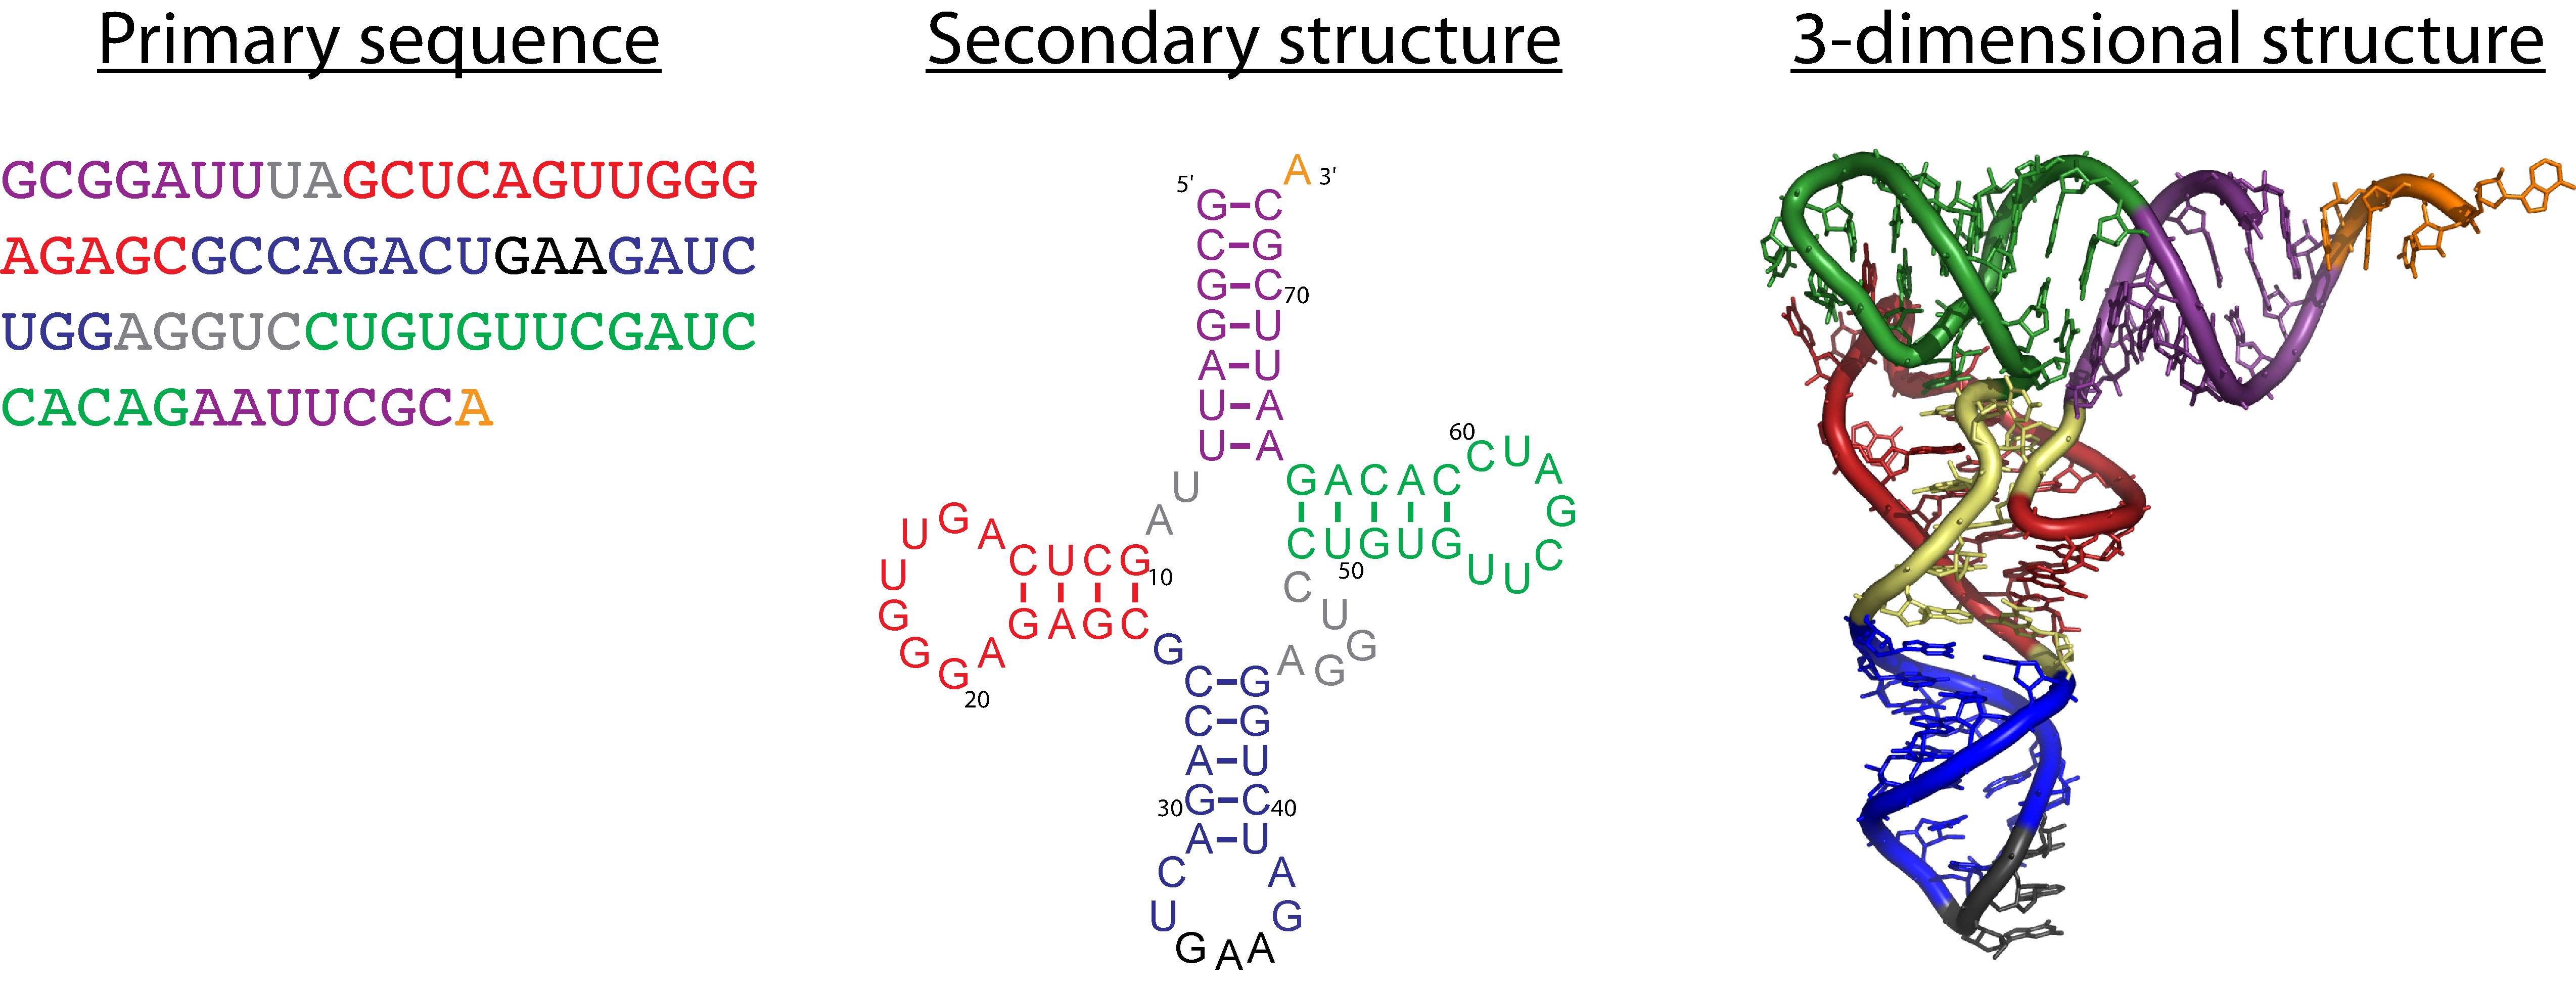
\includegraphics[width=10.5in]{figs/trna-123}
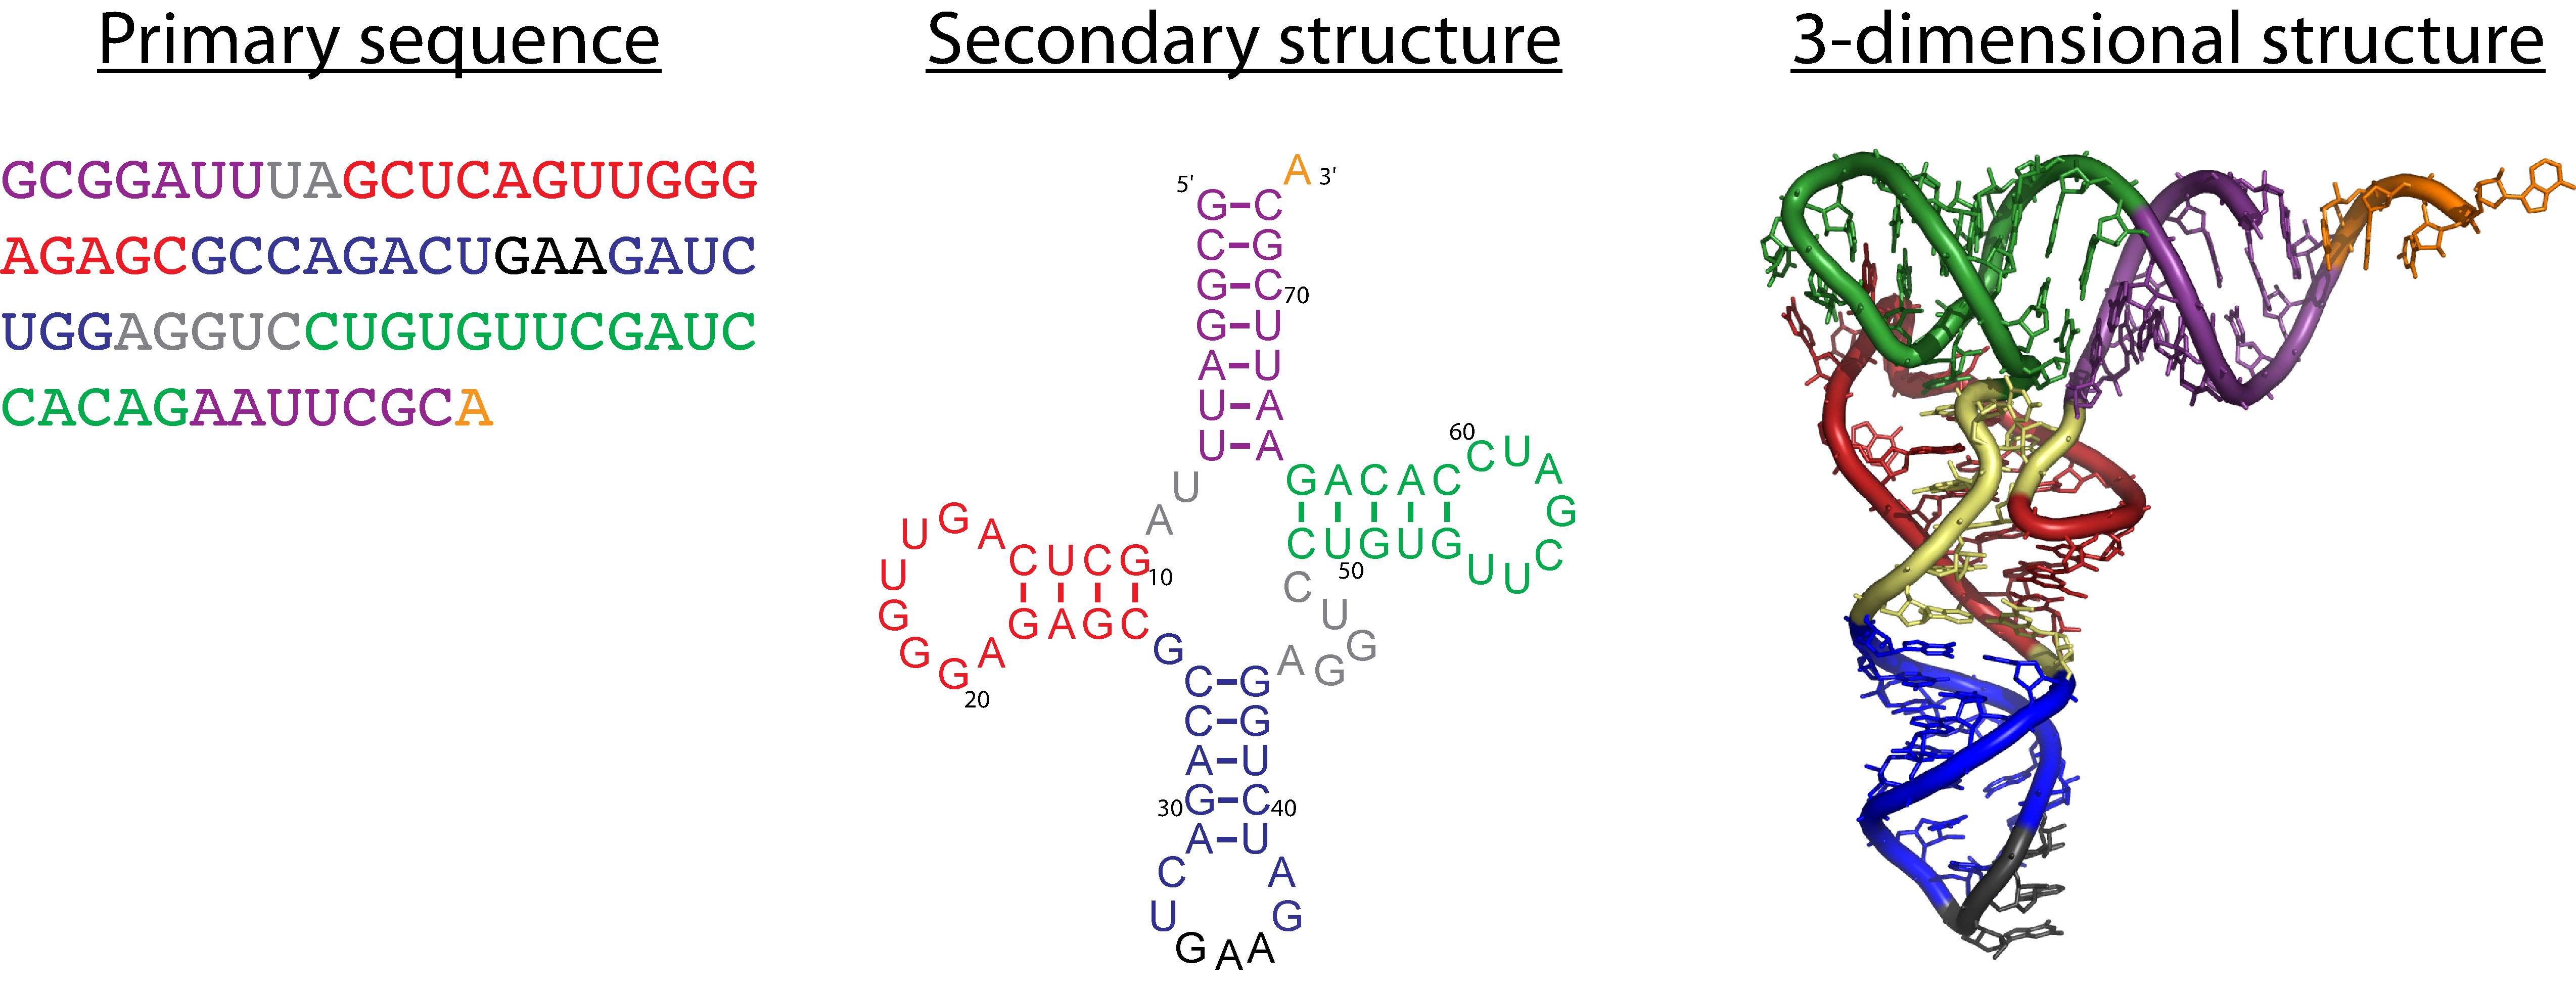
\includegraphics[width=9in]{figs/trna-123}

\end{center}

\vfill

\end{slide}
%%%%%%%%%%%%%%%%%%%%%%%%%%%%%%%%%%%%%%%%%%%%%%%%%%%%%%%%%%%%%%
\begin{slide}
\begin{center}
{\bf Most proteins and RNAs adopt a conserved 3-dimensional 
  structure that is responsible for their function in the cell}

\medskip

Three representations of a transfer RNA:

%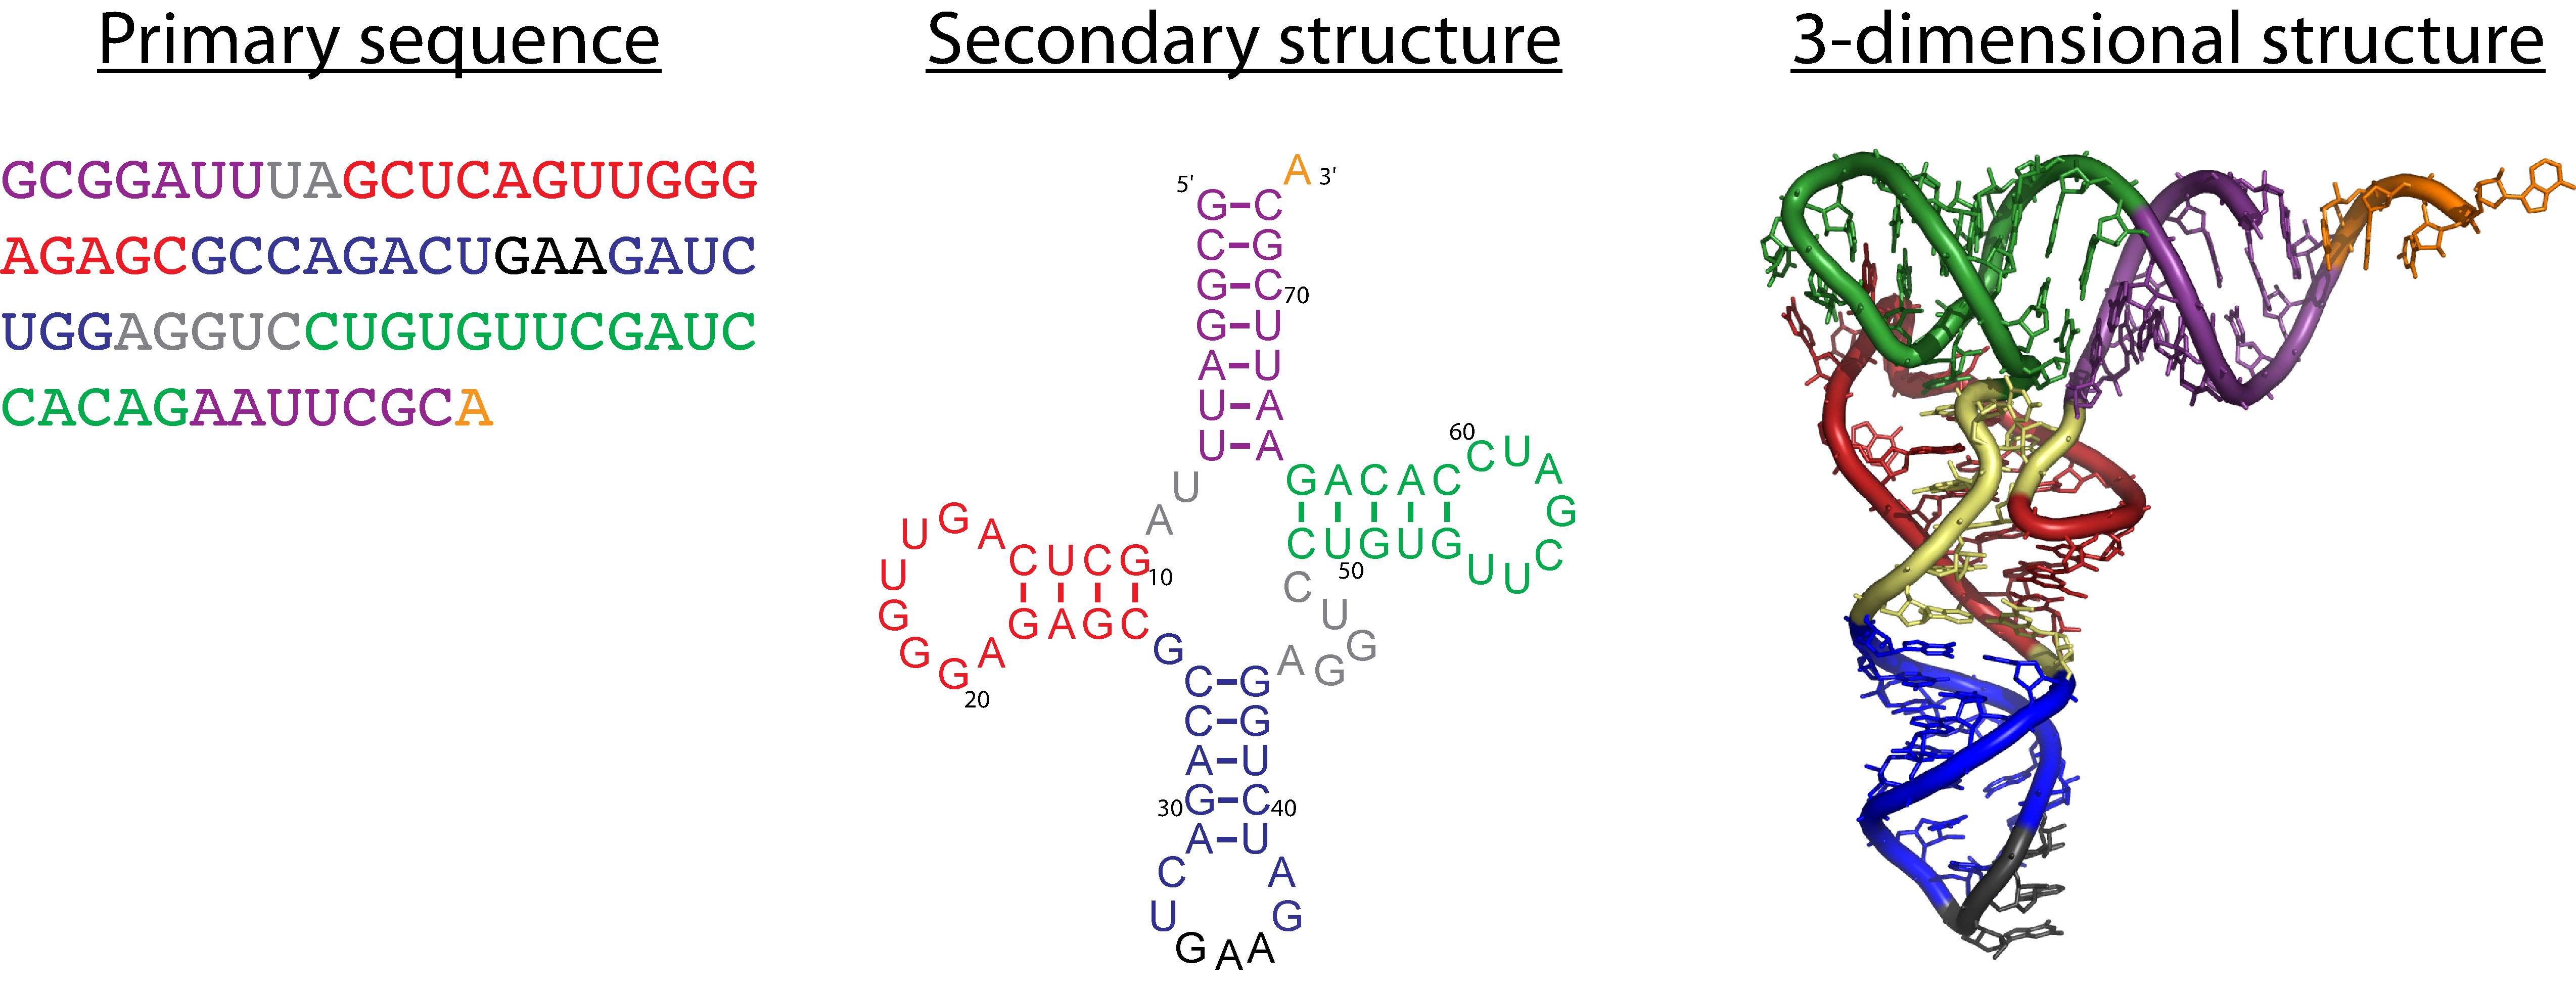
\includegraphics[width=10.5in]{figs/trna-123}
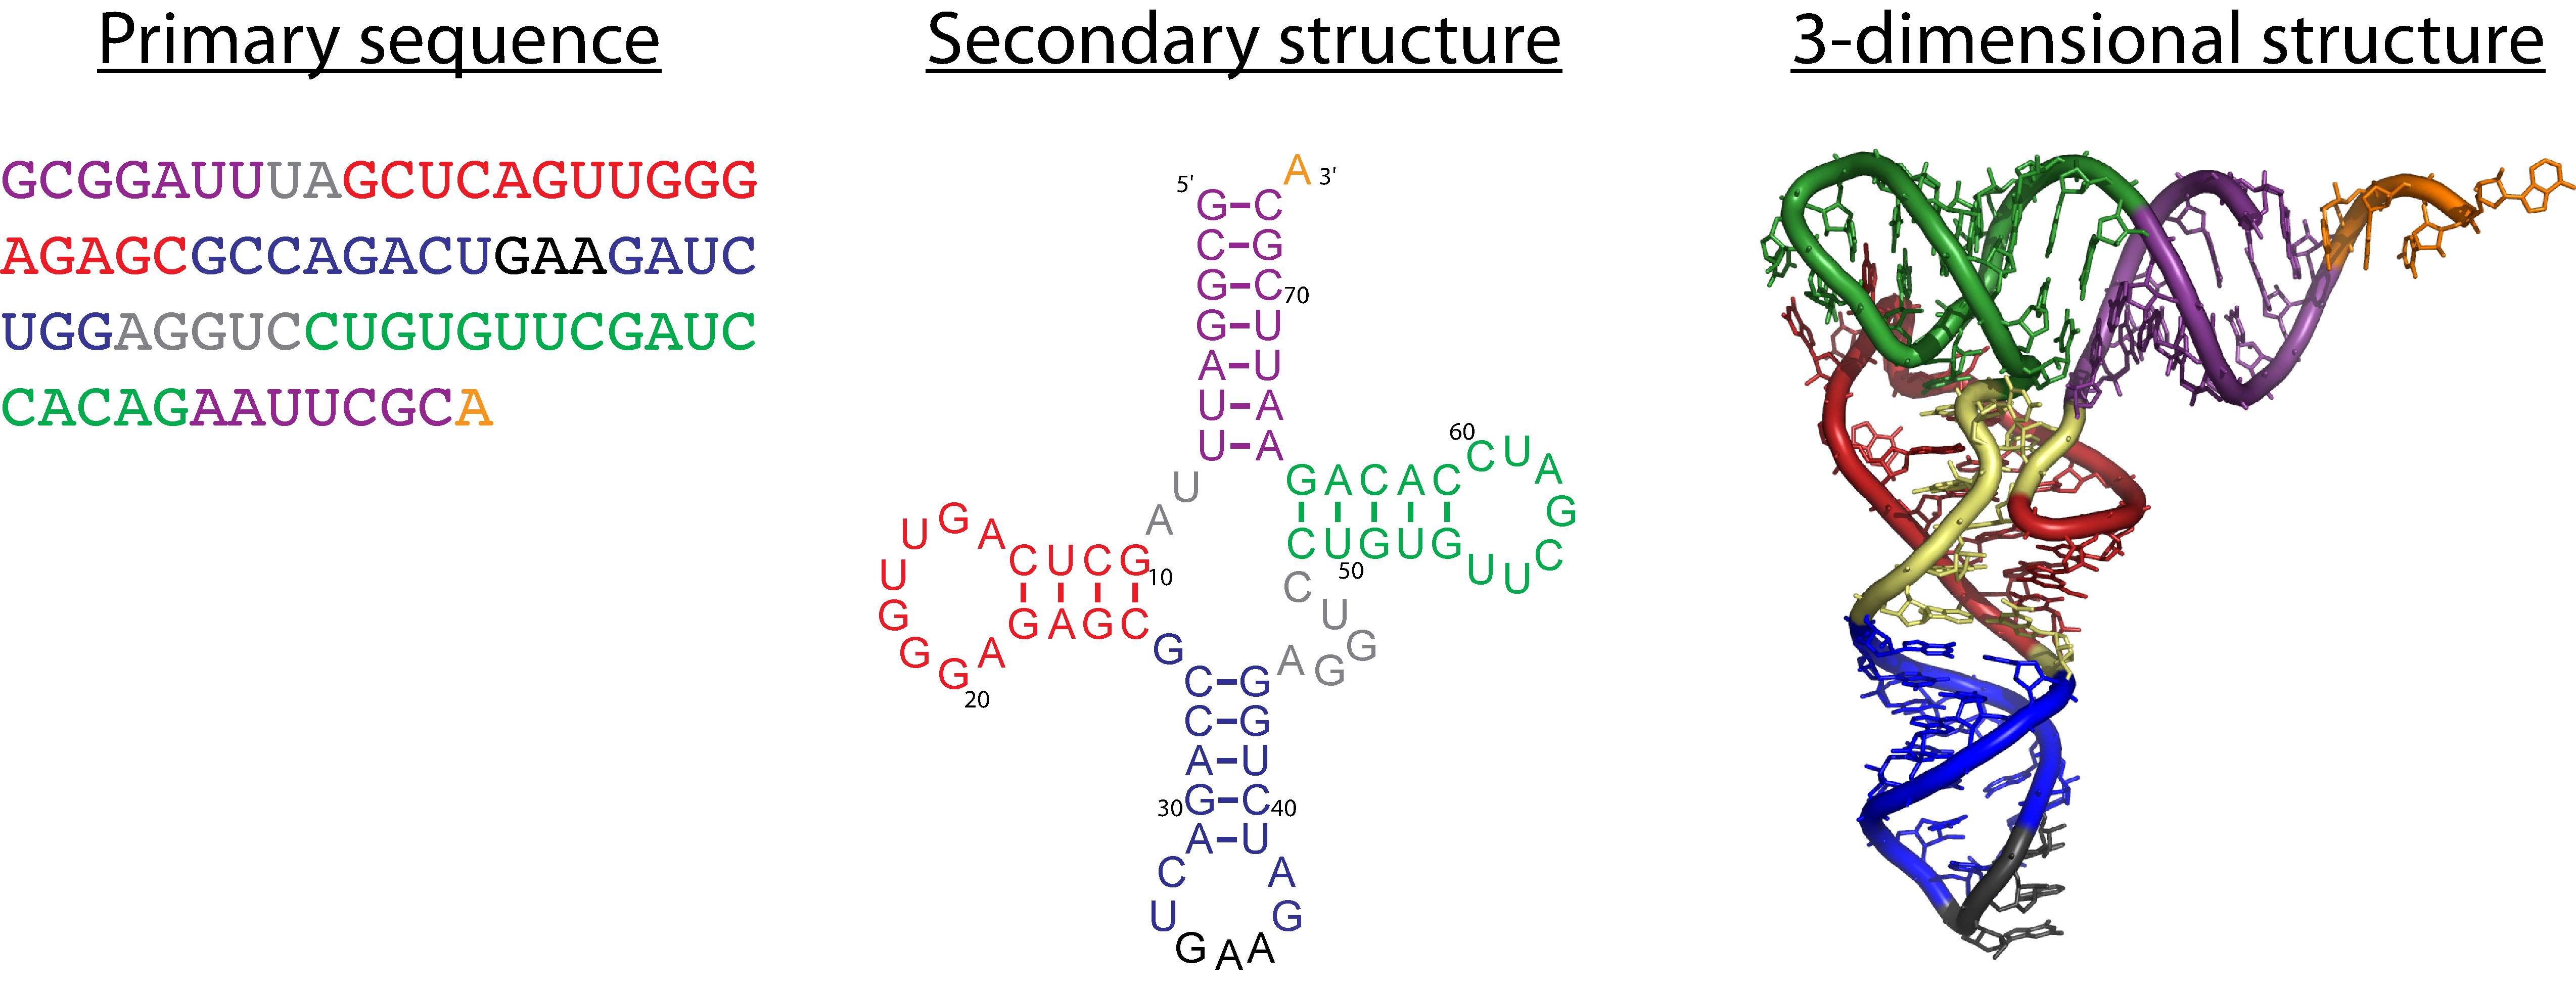
\includegraphics[width=9in]{figs/trna-123}

{\bf BLAST:} given a single sequence, search genomes for similar sequences.

%{\bf Homologous proteins and RNAs conserve \\ both sequence
%and structural features}

{\bf Homologous proteins and RNAs conserve different sequence \\
and structural features to different degrees.}
\end{center}

\vfill

\end{slide}
%%%%%%%%%%%%%%%%%%%%%%%%%%%%%%%%%%%%%%%%%%%%%%%%%%%%%%%%%%%%%
\begin{slide}
\begin{center}
%\textbf{Comparative analysis of sequence families}: \\
\textbf{Sequence conservation provides \\ information for homology searches}
%\emph{Functionally important sequence features are evolutionarily conserved.}
\medskip

%A simple, made-up RNA family:

%Evolution conserves functionally \\ important sequence features.

%Evolution conserves sequence \\ based on its functional importance.

Conservation levels vary across alignment columns.

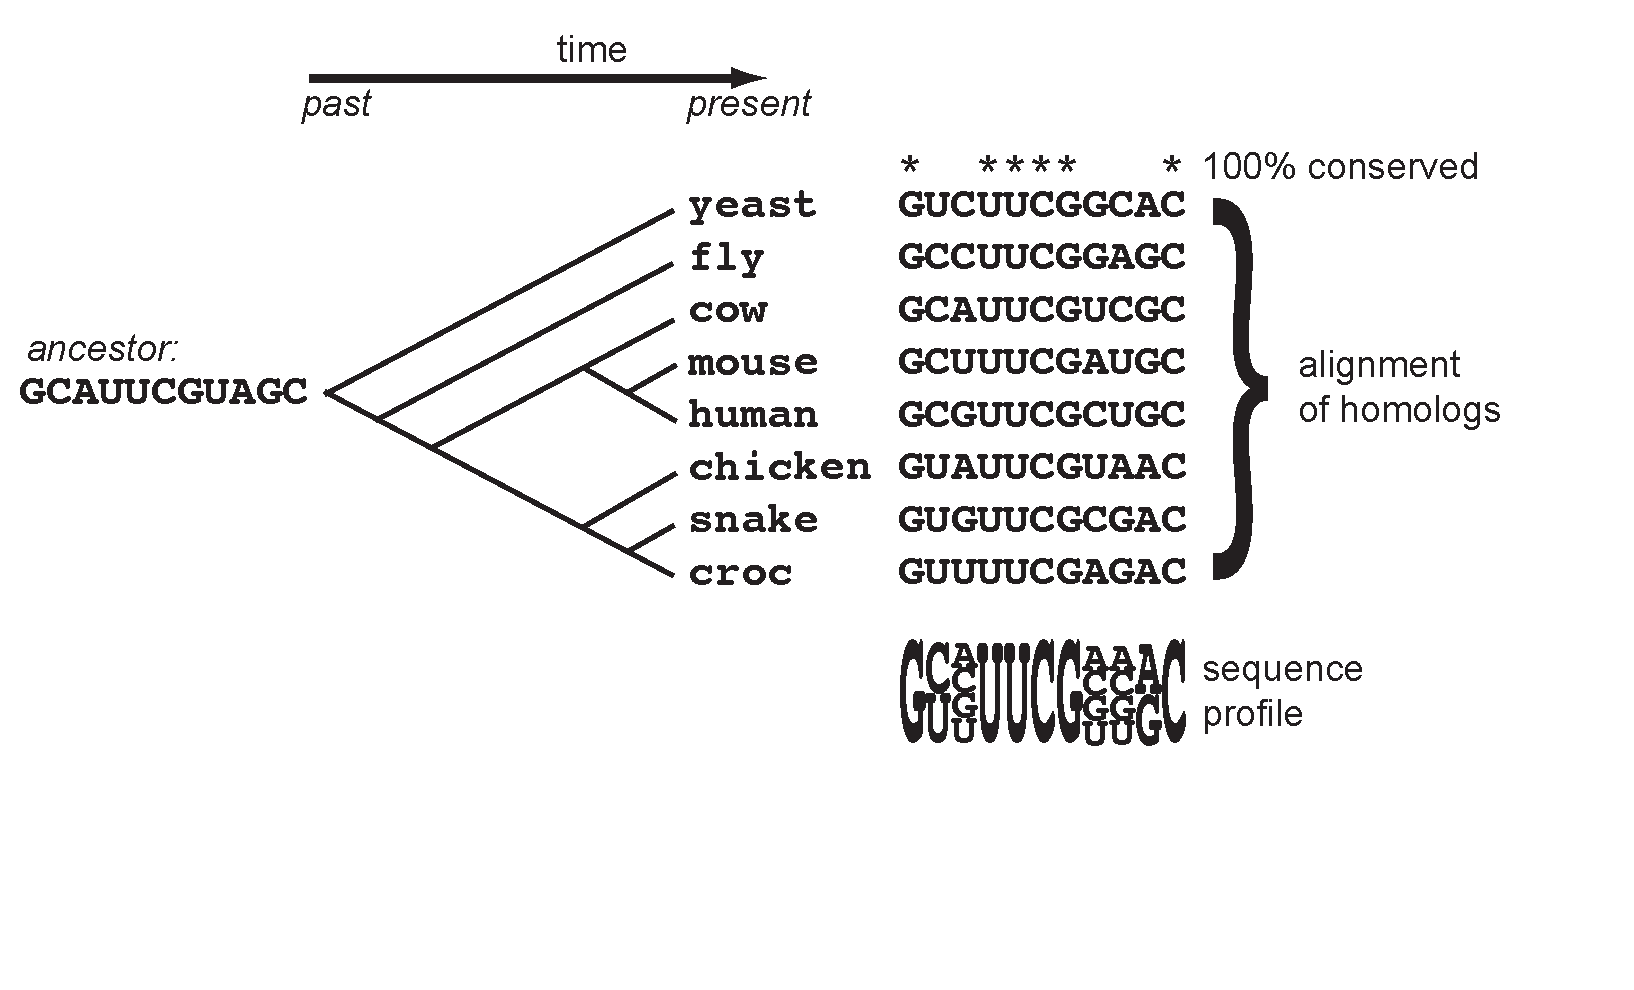
\includegraphics[width=10in]{figs/seqstructprofiles-seq1}
\end{center}

\vfill
\end{slide}
%%%%%%%%%%%%%%%%%%%%%%%%%%%%%%%%%%%%%%%%%%%%%%%%%%%%%%%%%%%%%%%%%%%%%%
\begin{slide}
\begin{center}
\textbf{Structure conservation provides additional information}
\medskip

Base-paired positions covary \\ to maintain Watson-Crick complementarity.

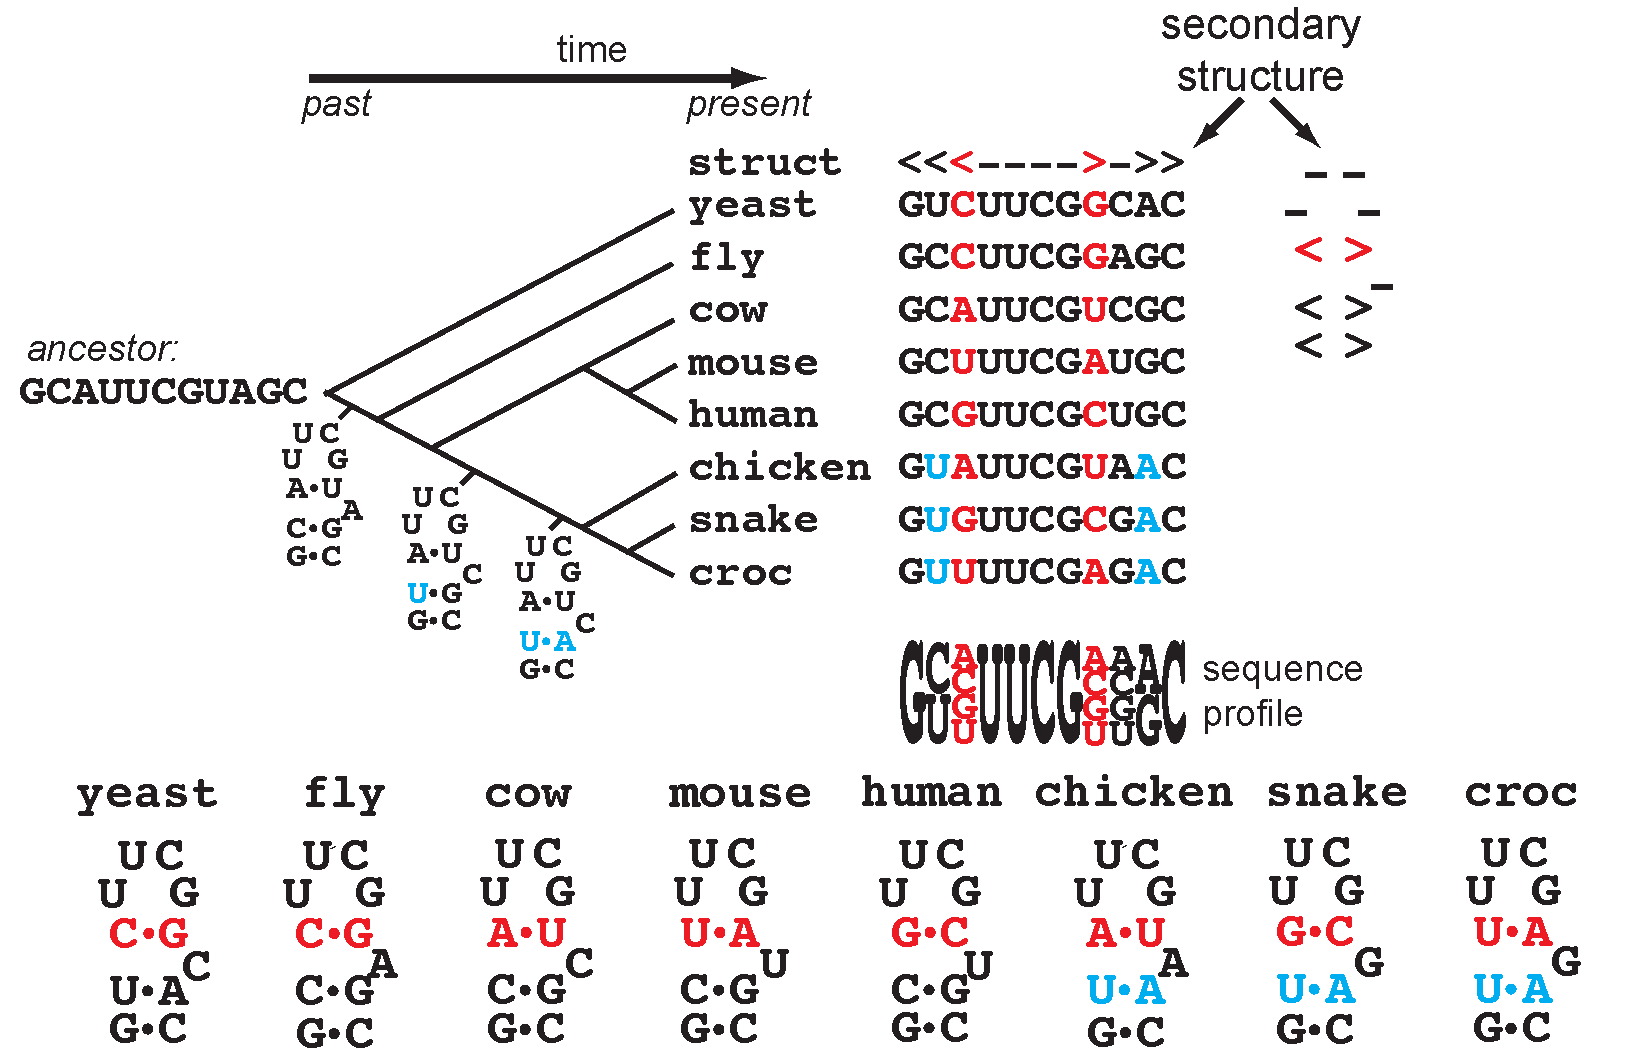
\includegraphics[width=10in]{figs/seqstructprofiles-struct2}
\end{center}

\vfill
\end{slide}
%%%%%%%%%%%%%%%%%%%%%%%%%%%%%%%%%%%%%%%%%%%%%%%%%%%%%%%%%%%%%%%%%%%%%%%%%%
\begin{slide}
\begin{center}
\textbf{Amount of information in a profile can be measured in bits}
\medskip

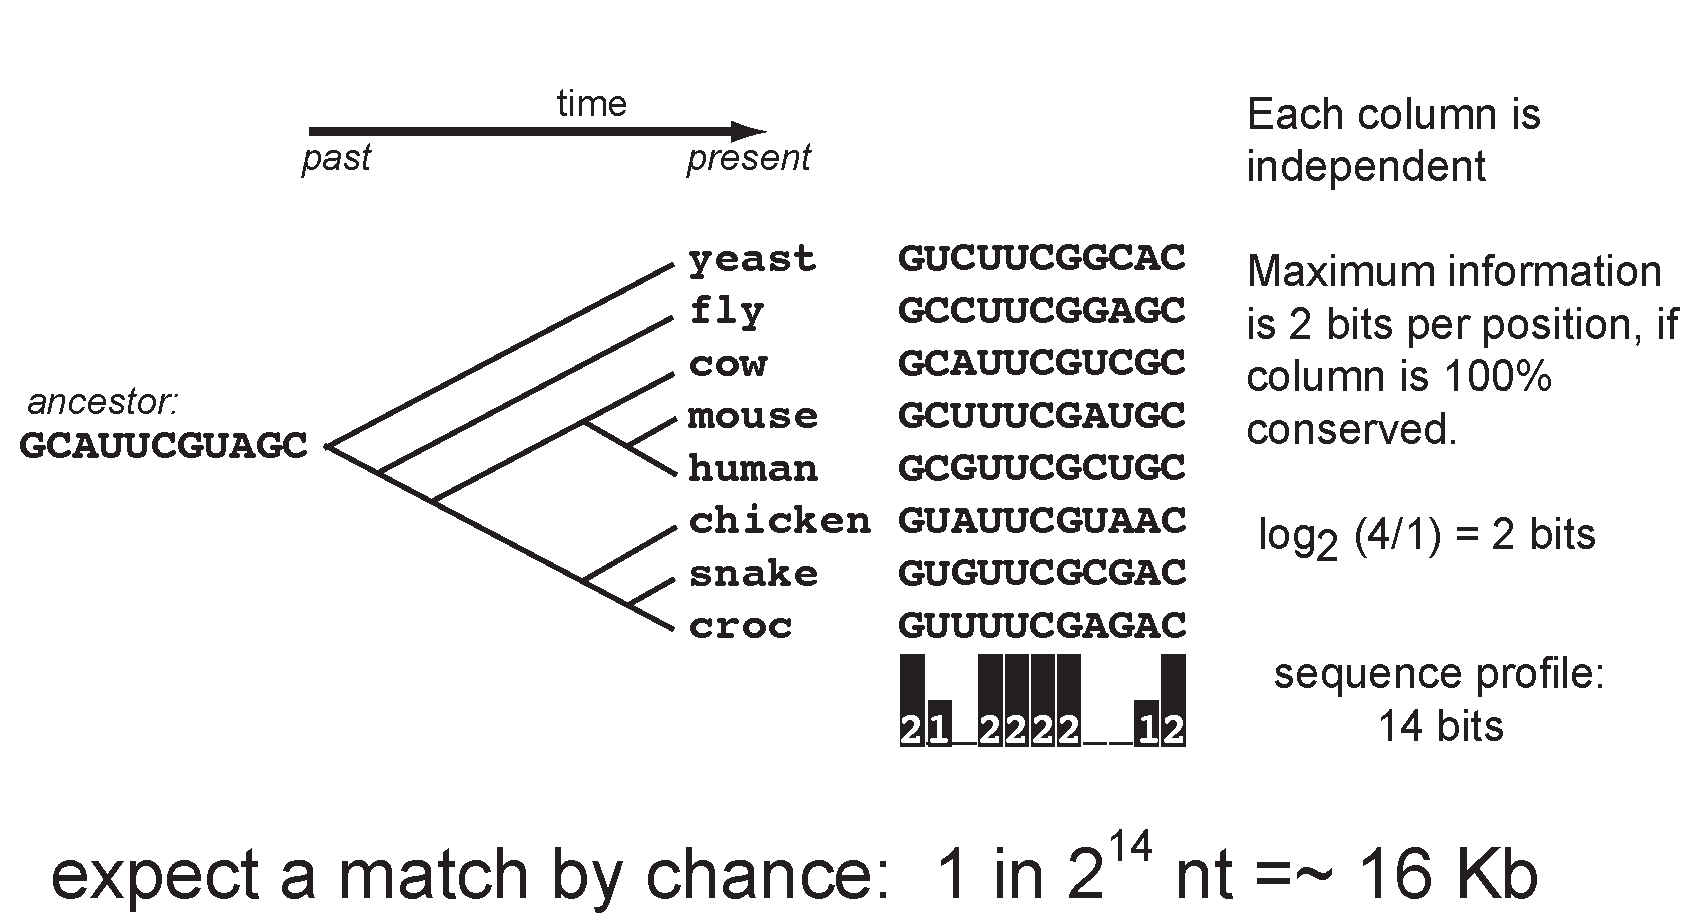
\includegraphics[width=9in]{figs/seqstructprofiles-2014-seqinfo}
\end{center}

\vfill
\end{slide}
%%%%%%%%%%%%%%%%%%%%%%%%%%%%%%%%%%%%%%%%%%%%%%%%%%%%%%%%%%%%%%%%%%%%%%%%%%
\begin{slide}
\begin{center}
\textbf{Structure contributes additional information from covariation}
\medskip

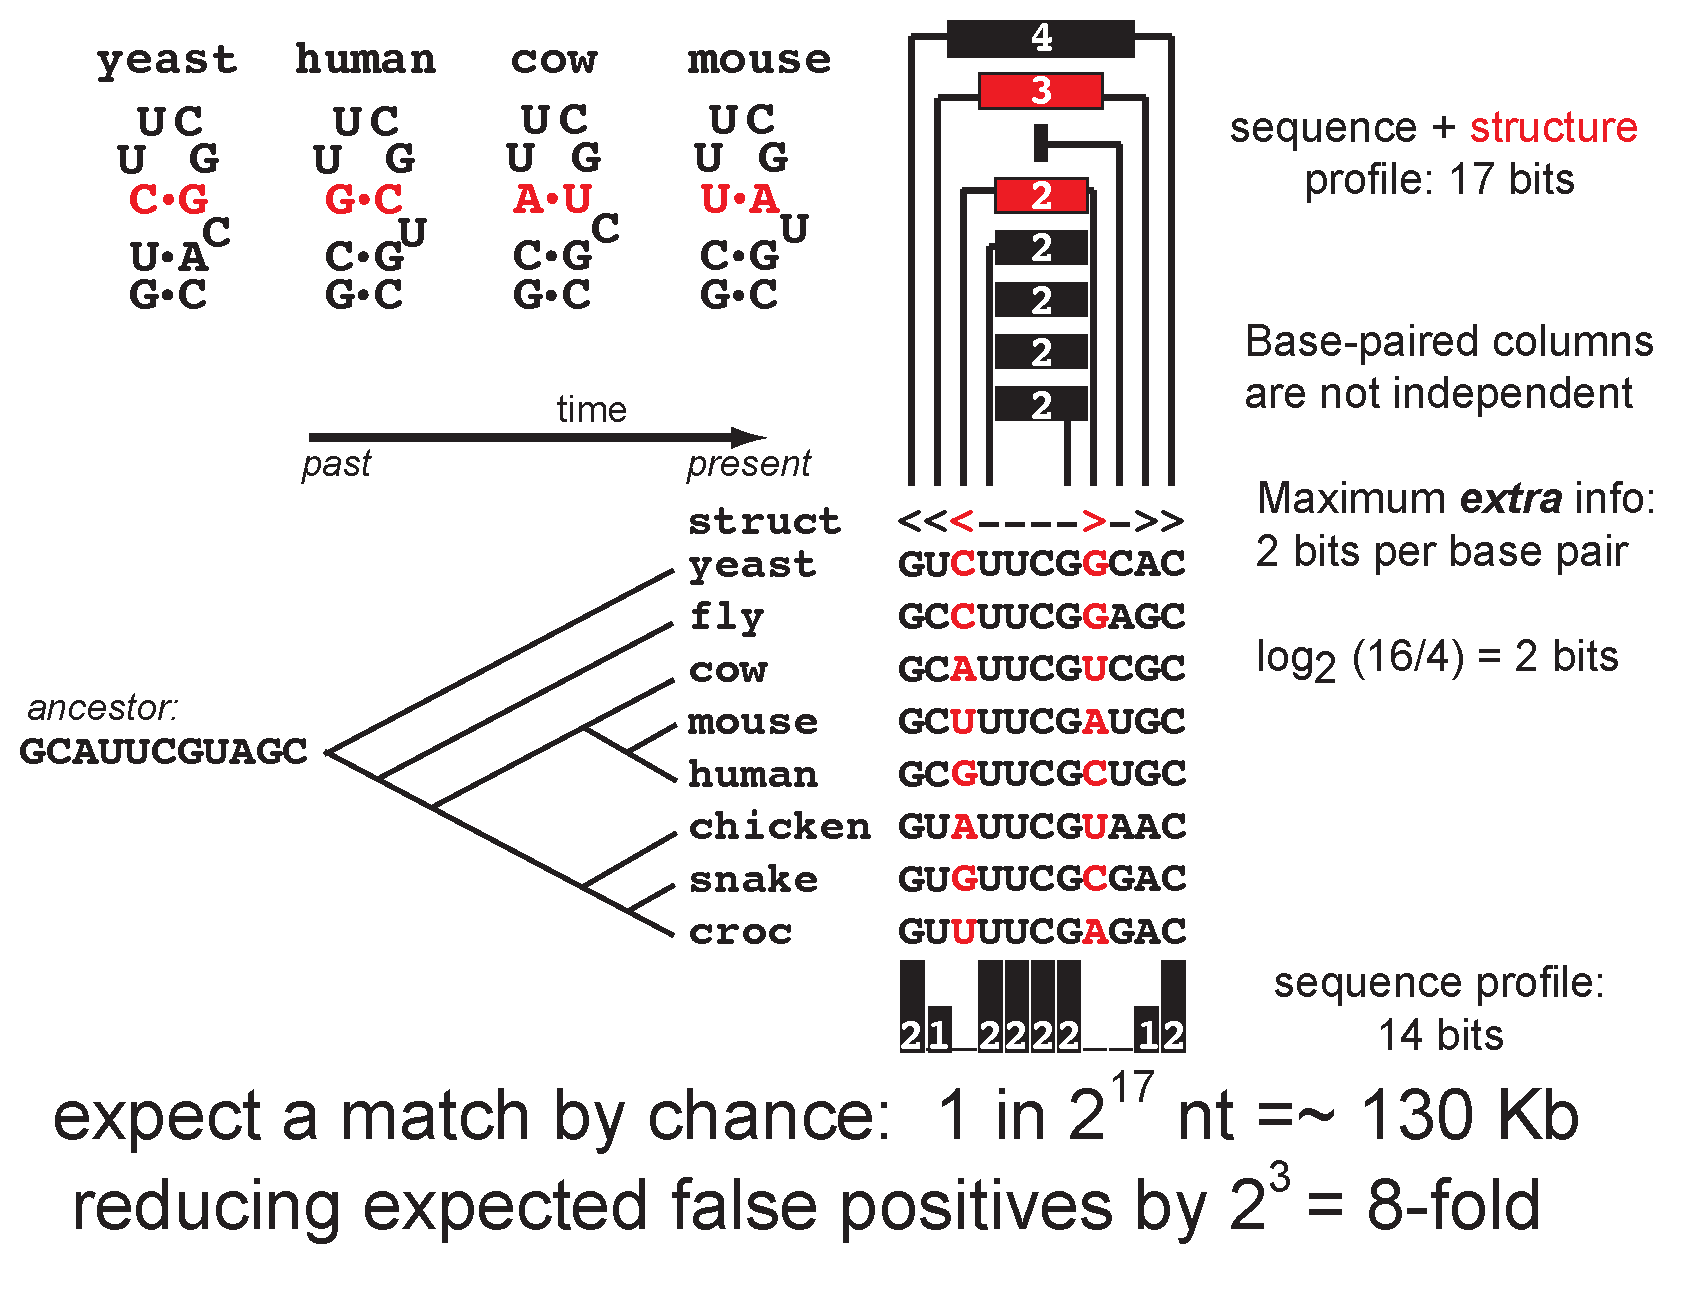
\includegraphics[width=9in]{figs/seqstructprofiles-2014-structinfo}
\end{center}

\vfill
\end{slide}
%%%%%%%%%%%%%%%%%%%%%%%%%%%%%%%%%%%%%%%%%%%%%%%%%%%%%%%%%%%%%%%%%%%%%%%%%%
\begin{slide}
\begin{center}
\textbf{Levels of sequence and structure conservation in RNA families}
\end{center}
\medskip

\begin{center}
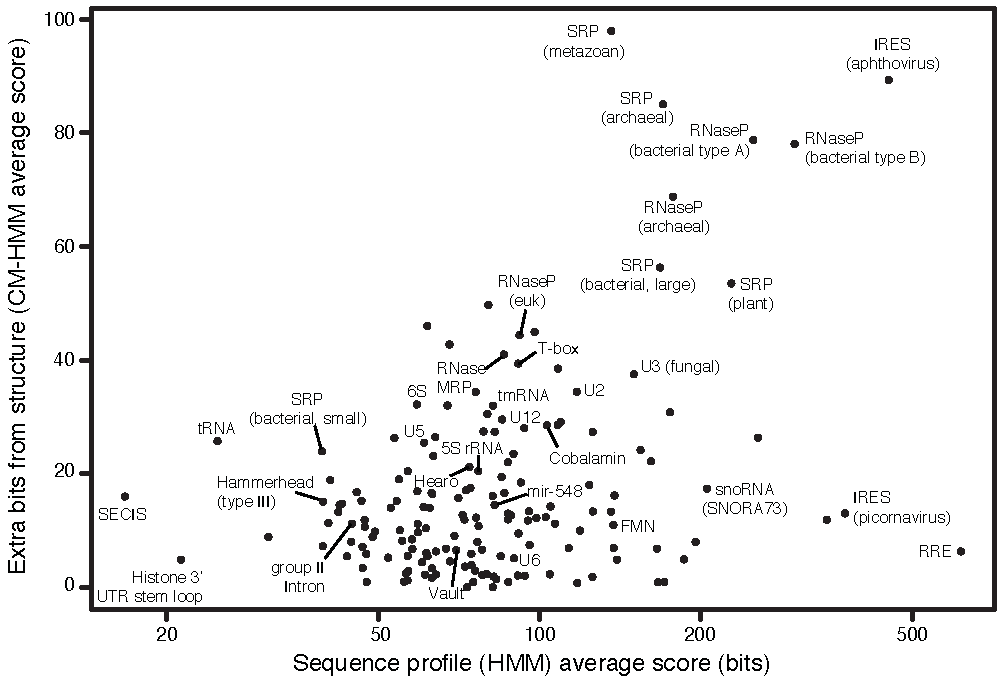
\includegraphics[height=6.5in]{figs/avgscores-rfam11}
\end{center}

\vfill

\end{slide}
%%%%%%%%%%%%%%%%%%%%%%%%%%%%%%%%%%%%%%%%%%%%%%%%%%%%%%%%%%%%%%%%%%%
\begin{slide}
\begin{center}
%\textbf{profile HMMs and covariance models}
\textbf{Eddy lab software for profile probabilistic models } (since 1994)
\end{center}
\medskip

\begin{center}
\small
\begin{tabular}{r|cc} 
%             &         & sequence \\
%             & sequence& and structure \\
%             & profiles& profiles \\ \hline
             & sequence & sequence and \\
             & profiles & structure profiles \\ \hline
  \\
  models     & profile HMMs     & {\color{red} covariance models (CMs)} \\ 
  \\
  software   & {\sc HMMER}      & {\sc Infernal} \\ 
  \\
  main use   & proteins,         & structural RNAs \\ 
             & repetitive DNA elements &  \\
  \\
  databases  & {\sc Pfam} and \sc{Dfam}       & {\sc Rfam} \\
             & (14831 and 1132 entries) & (2450 families) \\
  \\
%  primary sequence & yes & yes \\
%  \\
%  secondary structure & no & yes \\
%  \\
%  algorithms & Viterbi, Forward & CYK, Inside \\
%%             & Forward & Inside \\
%             &         & \\
%  complexity & $O(LN)$ & $O(LN^{2} log N)$ \\
%  \\
  performance& faster but    & slower but    \\
  for RNAs   & less accurate & more accurate \\
\end{tabular}

%\hspace{1.2in}\includegraphics[height=2in]{figs/hmmer_logo}\hspace{1.05in}\includegraphics[height=2.6in]{figs/infernal_logo}
\hspace{1.2in}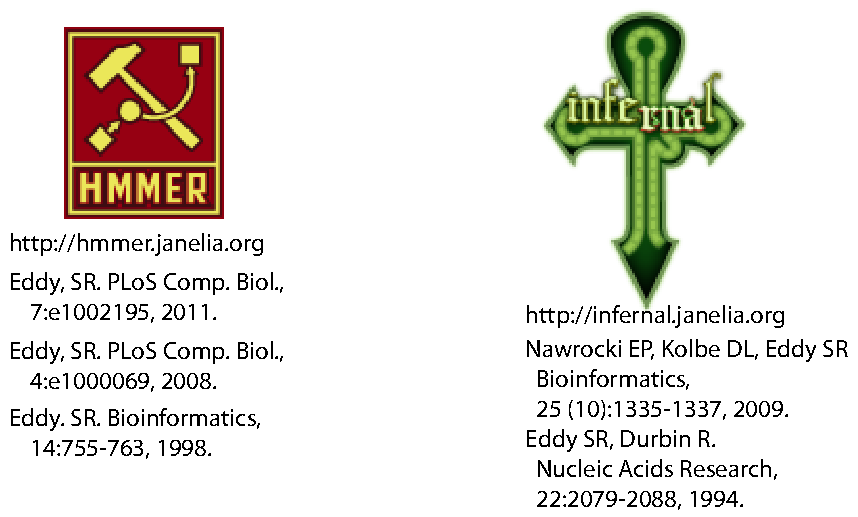
\includegraphics[height=2.7in]{figs/hmmer-infernal-refs}

\end{center}

\vfill

\end{slide}
%%%%%%%%%%%%%%%%%%%%%%%%%%%%%%%%%%%%%%%%%%%%%%%%%%%%%%%%%%%%%%%
\begin{slide}
\begin{center}
\textbf{Is the added complexity worth it? \\
  RMARK: a challenging \underline{internal} RNA homology search \\
  benchmark for use during Infernal development}
\end{center}
\medskip
\begin{minipage}{7in}
\small
\begin{itemize}
\item
  RMARK construction - for each of the 1446 Rfam 10 seed alignments:
  \begin{itemize}
%  \item
%    remove sequences $<$ 70\% average family length
  \item 
    cluster sequences by sequence identity \\ given the alignment
  \item 
    look for a \textcolor{blue}{training} cluster and
    \textcolor{red}{testing} cluster such that: 
    \begin{itemize}
    \item
      no \textcolor{blue}{training}/\textcolor{red}{test} sequence pair is $>$ 60\% identical
    \item
      at least five sequences are in the \textcolor{blue}{training} set
    \end{itemize}
  \item
    filter \textcolor{red}{test} set so no two test seqs $>$ 70\% identical 
  \item
    %51 families qualify, with 450 \textcolor{red}{test} sequences
    106 families qualify, with 780 test sequences
  \item
    %\textcolor{red}{test} seqs are embedded in a 1 Mb pseudo-genome (25\% A,C,G,U)
    test seqs are embedded in a 10 Mb pseudo-genome of ``realistic'' base composition
%  \item
%    %    \textsc{BLAST}: family-pairwise search, each \textcolor{blue}{training} seq is used
%        \textsc{BLAST}: family-pairwise search, each \\ training sequence is used
%    as a separate query
%  \item
%    %\textsc{Infernal}: build 1 CM per family from \textcolor{blue}{training} set
%    \textsc{Infernal}: build 1 CM per family from \\ training alignment 
  \end{itemize}
\end{itemize}
\vspace{1.5in}
\end{minipage}
\hspace{0.1in}
\begin{minipage}{3.5in}
  Example: 
\vspace{0.2in}

\begin{center}
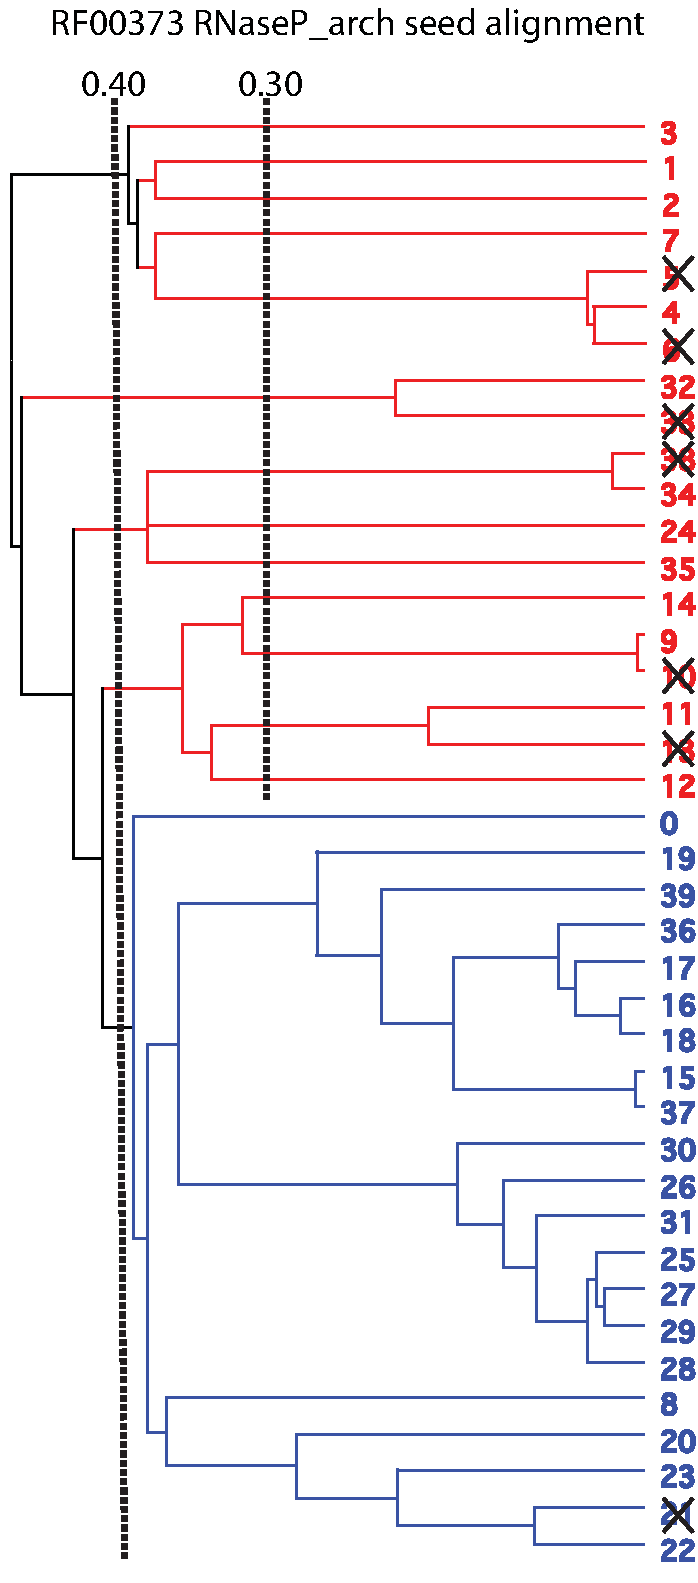
\includegraphics[height=5.5in]{figs/u8-RF00373-tree}

\end{center}
\end{minipage}
\end{slide}
%%%%%%%%%%%%%%%%%%%%%%%%%%%%%%%%%%%%%%%%%%%%%%%%%%%%%%%%%%%%%%%%%%%%%%
\begin{slide}
\begin{center}

\textbf{Infernal outperforms primary-sequence based methods on our
  benchmark (and others\footnote{Freyhult EK, Bollback JP, Gardner
    PP. Genome Res. 2007 17: 117-125.}, not shown)}

\end{center}
\medskip

\center{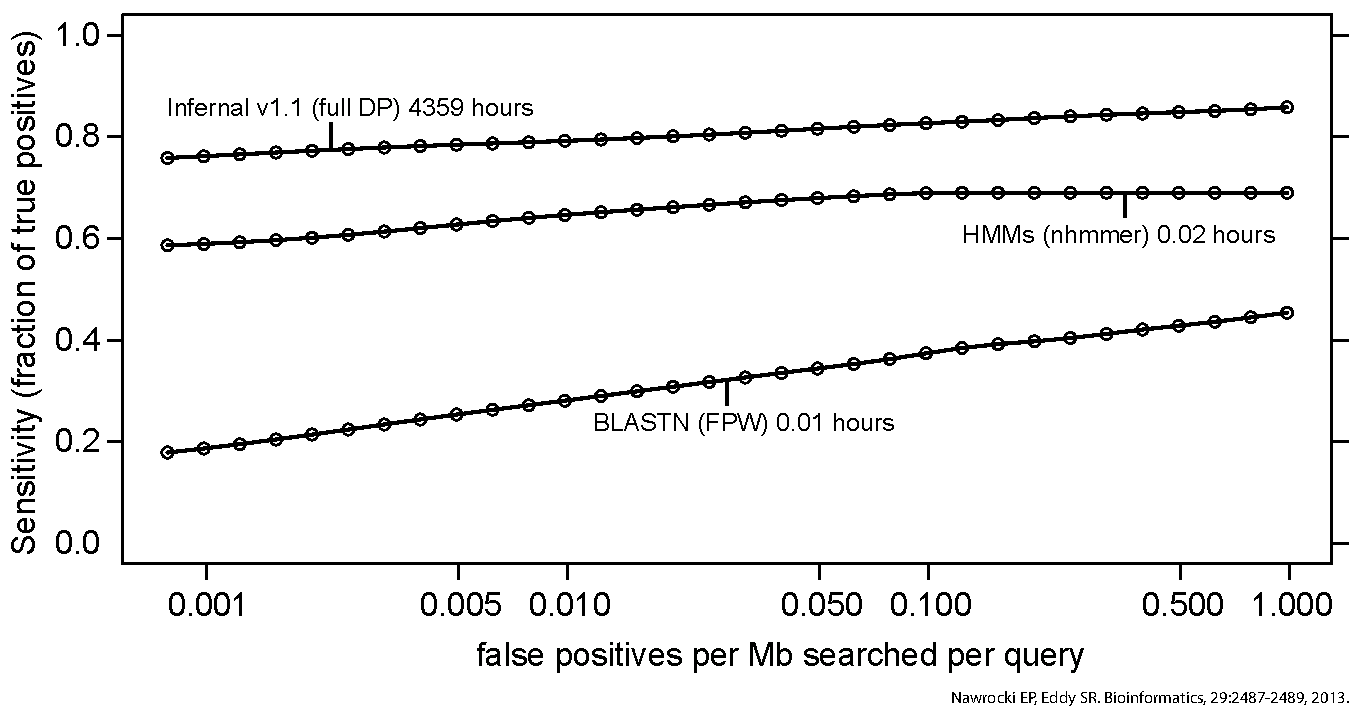
\includegraphics[width=10in]{figs/roc-talk-rcb-2014-1}}

\vfill 
\end{slide}
%%%%%%%%%%%%%%%%%%%%%%%%%%%%%%%%%%%%%%%%%%%%%%%%%%%%%%%%%%%%%%%%%%%%%%
\begin{slide}
\begin{center}
\textbf{Exploit sequence-based conservation using HMM filters}
\end{center}

\center{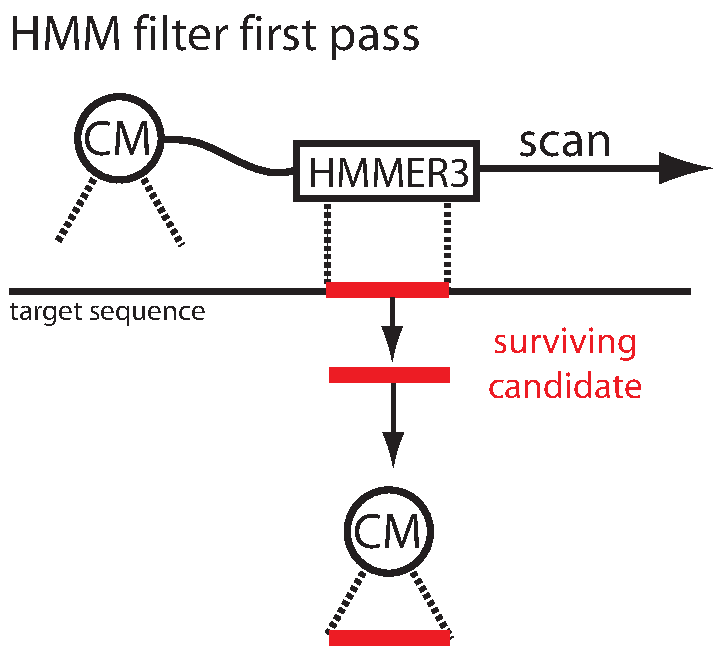
\includegraphics[height=6in]{figs/filter-2014-1}}

\vfill
\end{slide}
%%%%%%%%%%%%%%%%%%%%%%%%%%%%%%%%%%%%%%%%%%%%%%%%%%%%%%%%%%%%%%%%%%%%%%%%%%
\begin{slide}
\begin{center}

\textbf{Optimal alignment to an HMM}

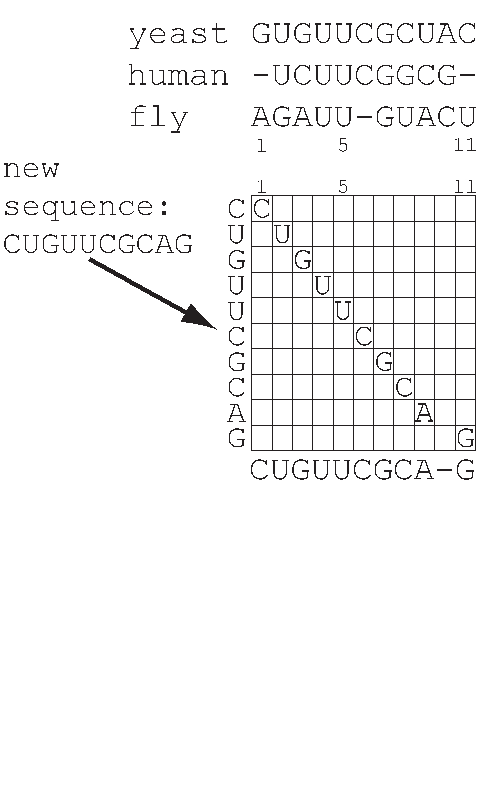
\includegraphics[height=6in]{figs/hmm_alignment2_layer2}
\end{center}

\vfill
\end{slide}
%%%%%%%%%%%%%%%%%%%%%%%%%%%%%%%%%%%%%
%%%%%%%%%%%%%%%%%%%%%%%%%%%%%%%%%%%%%%%%%%%%%%%%%%%%%%%%%%%%%%%%%%%%%%%%%%
\begin{slide}
\begin{center}

\textbf{Posterior decoding of an HMM alignment gives confidence estimates}

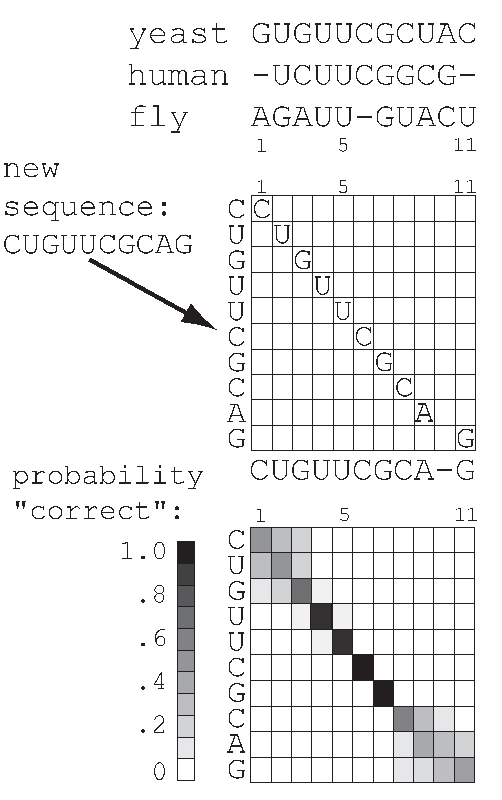
\includegraphics[height=6in]{figs/hmm_alignment2_layer3}
\end{center}

\vfill
\end{slide}
%%%%%%%%%%%%%%%%%%%%%%%%%%%%%%%%%%%%%
\begin{slide}
\begin{center}

\textbf{HMM bands accelerate CM alignment}
\end{center}
\medskip
\small
\begin{itemize}
\item
\textbf{main idea:} eliminate potential alignments the HMM tells us are very improbable
\end{itemize}
\begin{center}
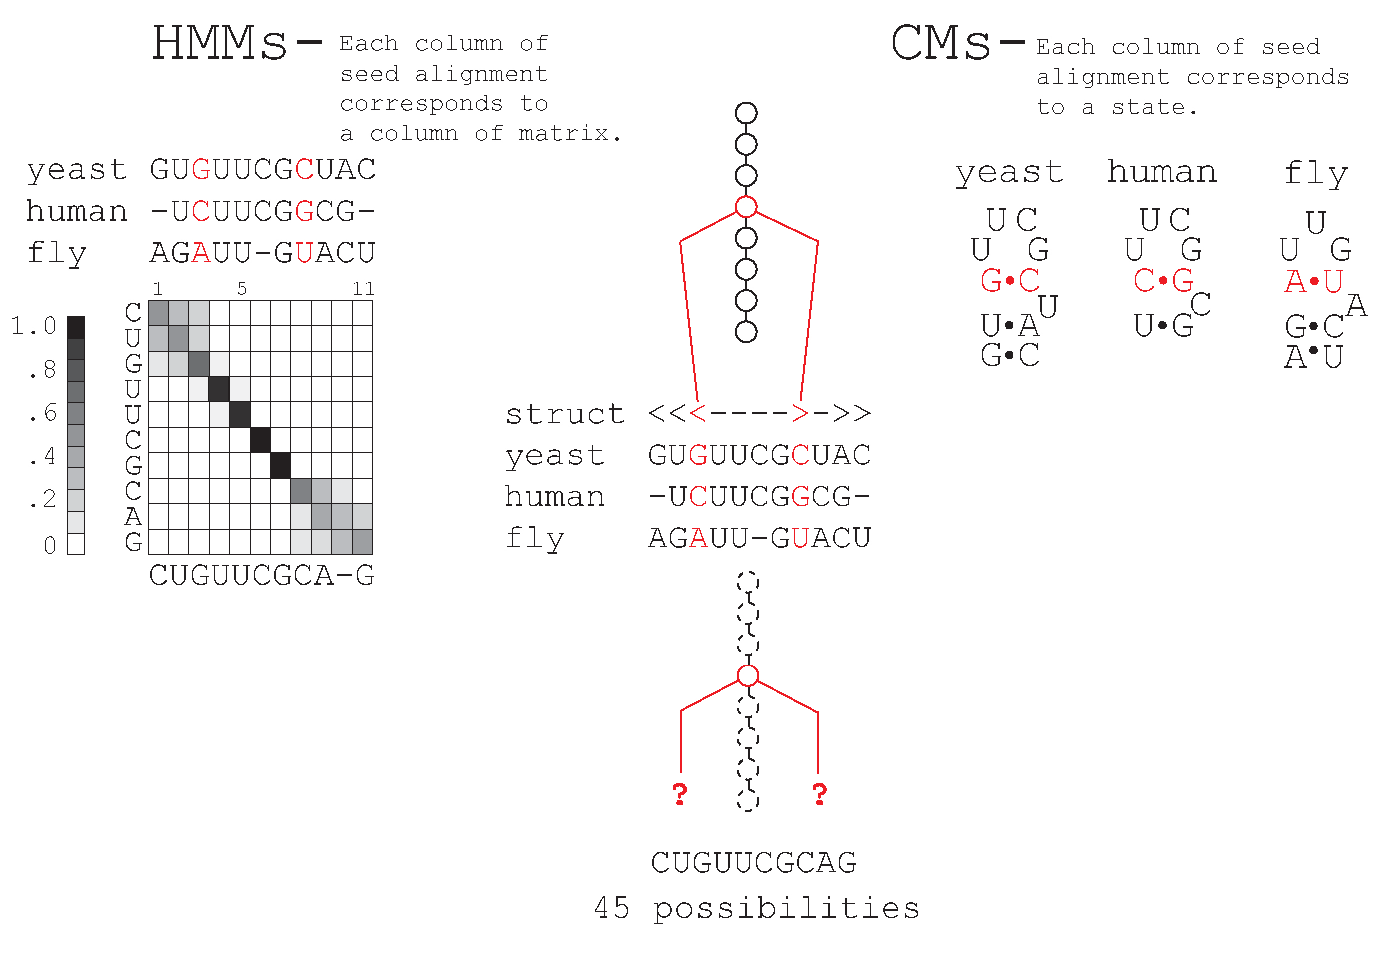
\includegraphics[width=8in]{figs/post_hmm_to_cm_map2_layer14}
\end{center}
\vfill
\end{slide}
%%%%%%%%%%%%%%%%%%%%%%%%%%%%%%%%%%%%%%%%%%%%%%%%%%%%%%%%%%%%%%%%%%%%%%
\begin{slide}
\begin{center}

\textbf{HMM bands accelerate CM alignment}
\end{center}
\medskip
\small
\begin{itemize}
\item
\textbf{main idea:} eliminate potential alignments the HMM tells us are very improbable
\end{itemize}
\begin{center}
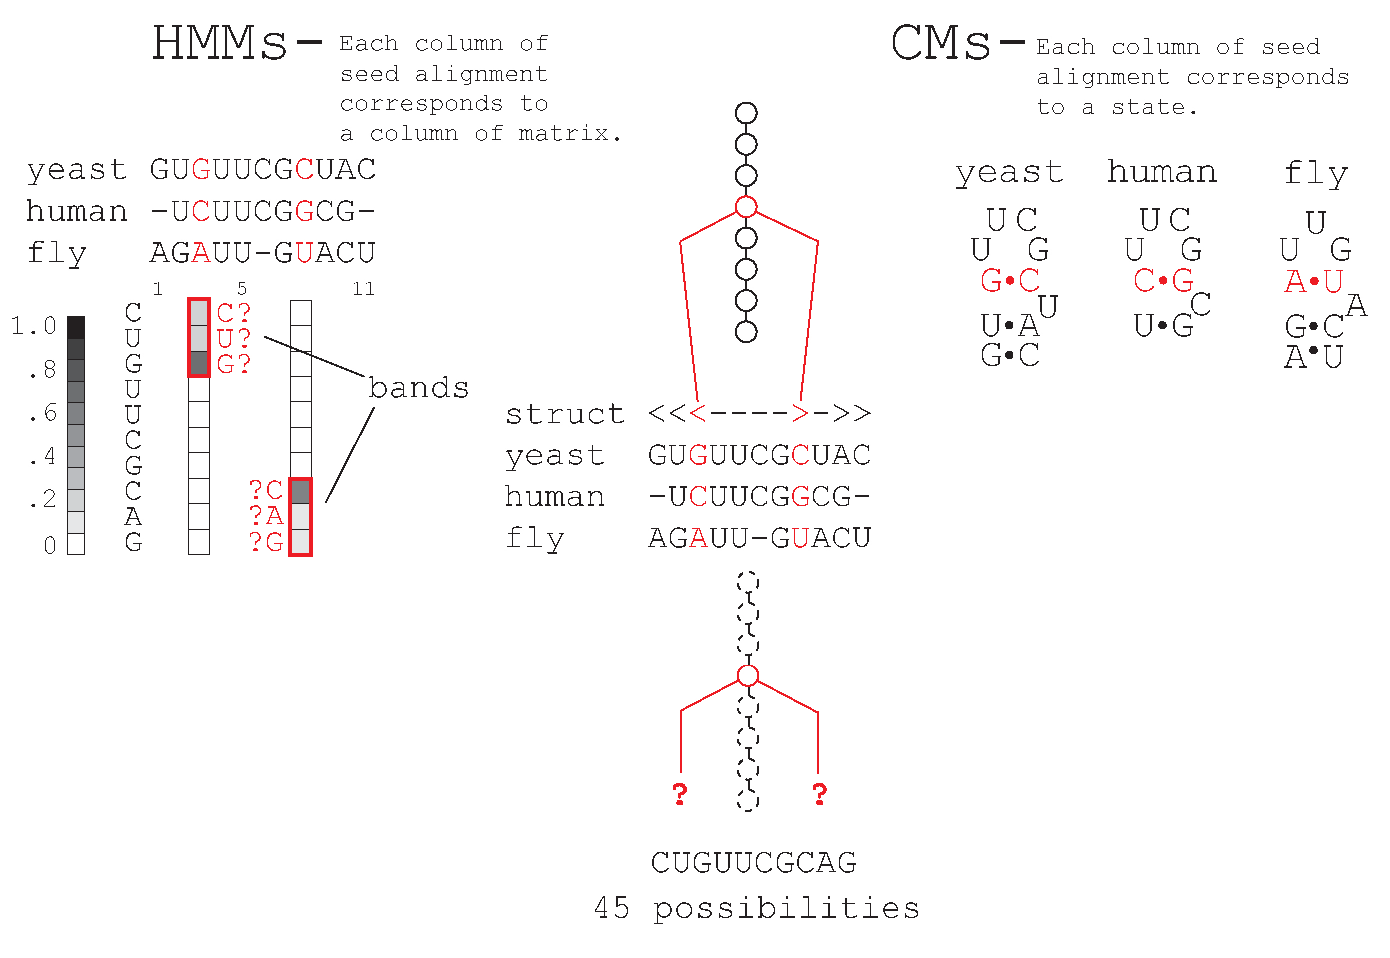
\includegraphics[width=8in]{figs/post_hmm_to_cm_map2_layer15}
\end{center}
\vfill
\end{slide}
%%%%%%%%%%%%%%%%%%%%%%%%%%%%%%%%%%%%%%%%%%%%%%%%%%%%%%%%%%%%%%%%%%%%%%%%%%
\begin{slide}
\begin{center}

\textbf{HMM bands accelerate CM alignment}
\end{center}
\medskip
\small
\begin{itemize}
\item
\textbf{main idea:} eliminate potential alignments the HMM tells us are very improbable
\end{itemize}
\begin{center}
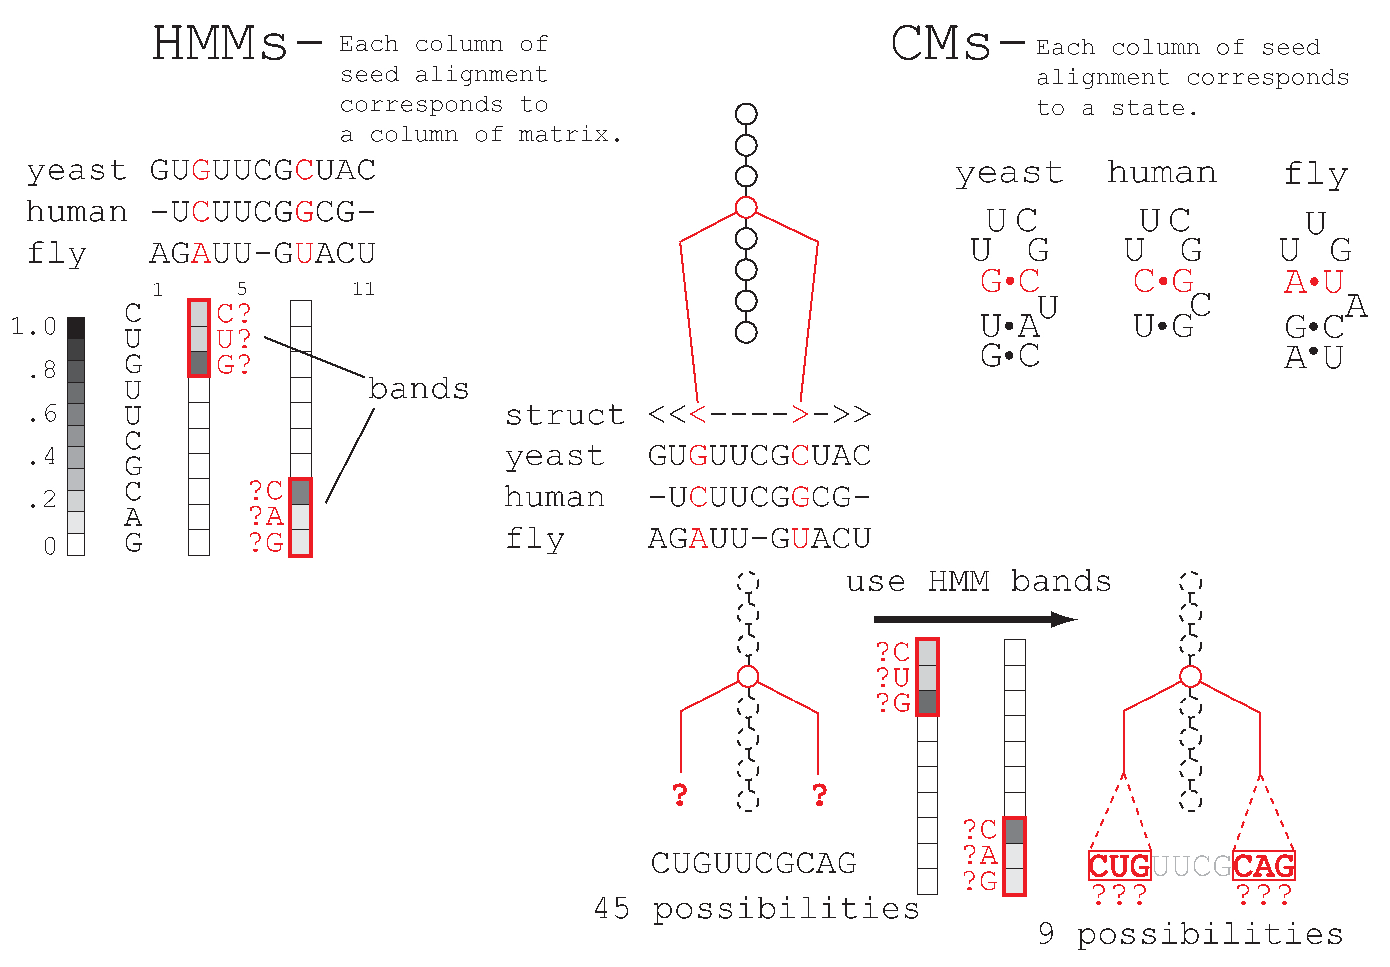
\includegraphics[width=8in]{figs/post_hmm_to_cm_map2_layer16}
\end{center}
\vfill
\end{slide}
%%%%%%%%%%%%%%%%%%%%%%%%%%%%%%%%%%%%%%%%%%%%%%%%%%%%%%%%%%%%%%%%%%%%%%
\begin{slide}
\begin{center}
\textbf{Use HMMs as filters and to constrain CM alignment}
\end{center}

\center{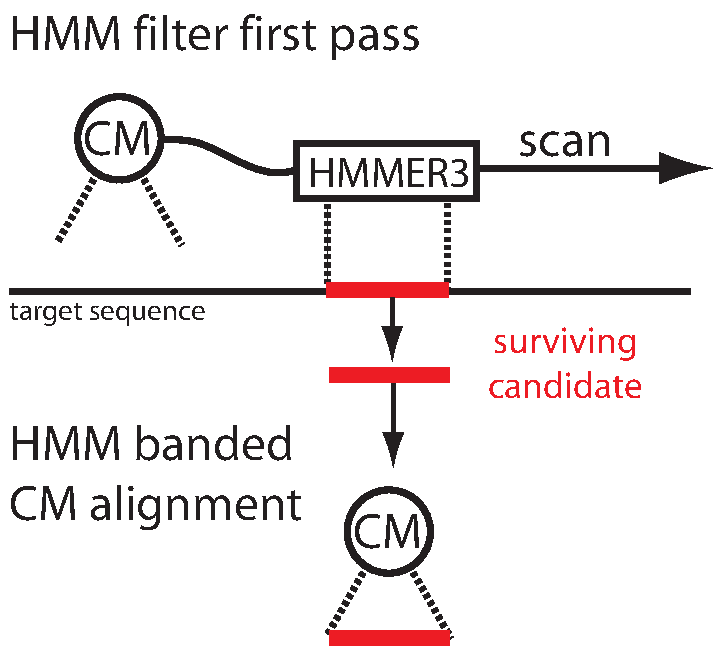
\includegraphics[height=6in]{figs/filter-2014-2}}

\vfill
\end{slide}
%%%%%%%%%%%%%%%%%%%%%%%%%%%%%%%%%%%%%%%%%%%%%%%%%%%%%%%%%%%%%%%%%%%%%%%%%%
\begin{slide}
\begin{center}

\textbf{HMM-based acceleration makes Infernal 10,000 times faster}

\end{center}
\medskip

\center{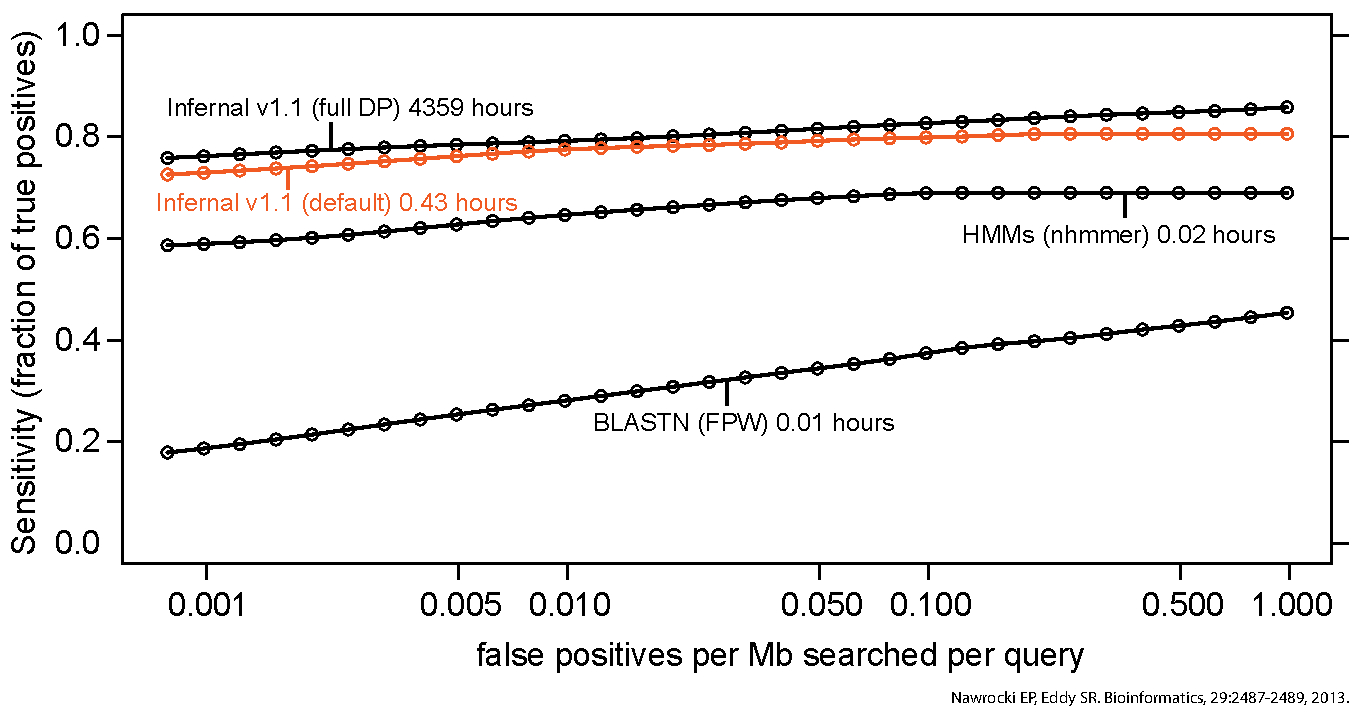
\includegraphics[width=10in]{figs/roc-talk-rcb-2014-2}}

\vfill 
\end{slide}
%%%%%%%%%%%%%%%%%%%%%%%%%%%%%%%%%%%%%%%%%%%%%%%%%%%%%%%%%%%%%%%%%%%%%%
\begin{slide}
\begin{center}

\textbf{Rfam's use of BLAST to accelerate Infernal search of large 270Gb Rfamseq database}

\end{center}

PICTURE HERE

\vfill 
\end{slide}
%%%%%%%%%%%%%%%%%%%%%%%%%%%%%%%%%%%%%%%%%%%%%%%%%%%%%%%%%%%%%%%%%%%%%%
\begin{slide}
\begin{center}

\textbf{Rfam 12.0: first release using Infernal without BLAST filters}

\end{center}

SUMMARY LINE FROM TABLE 1 HERE

\vfill 
\end{slide}
%%%%%%%%%%%%%%%%%%%%%%%%%%%%%%%%%%%%%%%%%%%%%%%%%%%%%%%%%%%%%%%%%%%%%%
\begin{slide}
\begin{center}

\textbf{An example family}

\end{center}

???

\vfill 
\end{slide}
%%%%%%%%%%%%%%%%%%%%%%%%%%%%%%%%%%%%%%%%%%%%%%%%%%%%%%%%%%%%%%%%%%%%%%
\begin{slide}
\begin{center}

\textbf{Rfam and Infernal-based genome/dataset annotation is simple}

\end{center}

???

\vfill 
\end{slide}
%%%%%%%%%%%%%%%%%%%%%%%%%%%%%%%%%%%%%%%%%%%%%%%%%%%%%%%%%%%%%%%%%%%%%%
\end{document}

